\documentclass[border=3pt]{standalone}
\usepackage{tikz}
\usepackage{amsmath}
\usepackage{amssymb}
\usepackage{ctex}
\usetikzlibrary{matrix, calc, positioning}
\usepackage{pgfplots}
\pgfplotsset{compat=1.18}

\begin{document}

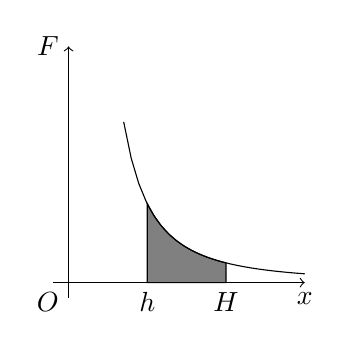
\begin{tikzpicture}
	\draw[->](-0.2,0)--(3,0)node[below]{$x$};
	\draw[->](0,-0.2)--(0,3)node[left]{$F$};
	\node[below left]at(0,0){$O$};
	\draw[fill=gray,domain=1:2] (1,0) -- plot({\x},{1/(\x)^2}) -- (2,0) -- cycle;
	\draw[domain=0.7:3] plot({\x}, {1/(\x)^2});
	\node[below]at(1,0){$h$};
	\node[below]at(2,0){$H$};
\end{tikzpicture}

\end{document}
